\documentclass{article}

\usepackage{graphicx}

\begin{document}

\title{Project Initial Design}
\author{Nicholas Muszynski}
\date{October 3, 2017}

\maketitle

\textbf{VR Fencing}
\newline

This project aims to replicate the sport of fencing within virtual reality, to provide players with an immersive experience as they spar against an AI opponent. To heighten the player's immersion in the game, movement of the player's body and control of their sword will be instrumental in playing and succeeding. The goals of this project are to deliver as immersive an experience as possible, with special focus on haptics (and the illusion of haptics) to provide satisfying feedback to the player. Likewise, this will be the main problem of the project, as it is paradoxical in nature: a primary concept of fencing is feeling the pressure of the one's blade against the other, and as such must be creatively approached to achieve this sensation in a virtual environment.\\

\newline

The user experience is intended to be simple: To move, the player physically moves. To attack or defend, the player holds their controller as they would a stick or other long object, and will swing to attack or put it in the way to defend themselves. By eliminating the need for any button or analog presses (except for menu interaction), it will encourage a natural flow of movement that is easy to understand. The user interface will also be minimalistic, only displaying necessary information when needed and keeping the player's view free of distractions and clutter.\\

\newline

Milestones:\\
1 - Basic compatibility/communication between software and hardware.\\
2 - Registration of physical movement and controls.\\
3 - Establish basic sword binding mechanics between physical and artificial players.\\
5 - Configure 'hitboxes', which determine when a player is hit.\\
5 - Configure AI for basic movement and strategies.\\
6 - Basic skeletal mesh animation systems.\\
7 - Improve AI and mechanics.\\
8 - Polishing any remaining minor features.\\

\newline

\begin{figure}[1]
\caption{Program structure concept}
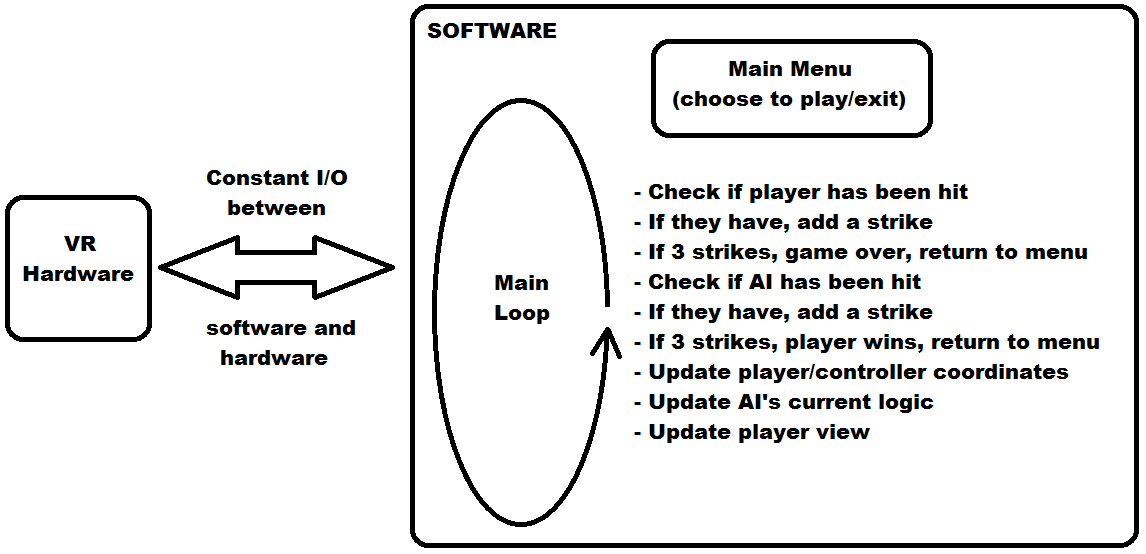
\includegraphics[width=\linewidth]{projectPicture.png}
\end{figure}

\end{document}